\section{Absorption models and the method of characteristics}
\label{sec:moc}

The chapter now changes tack. Everything so far has concerned a single population and the
chance that it survives; the remainder develops the analytical machinery for a second kind
of question, in which particles move between compartments and one wants the joint
distribution of the counts on either side.

The motivation is a modelling choice that arises as soon as more than one compartment is
present. Earlier work describes the birth--death dynamics of particles held inside a single
compartment that can rupture. Extending that description to several compartments sharing a
medium requires a decision about what happens when the first of them ruptures, because the
shared medium then acquires a potentially large cohort of particles available for
subsequent uptake by the remaining compartments. The analysis so far has assumed
\emph{immediate transfer}: the entire contents of a rupturing compartment relocate at once
into another compartment. That is a strong assumption. A more realistic alternative is an
\emph{absorption period}, in which absorption events redistribute the released cohort among
the remaining compartments, and birth, death and rupture resume only when every particle
has been taken up. Working towards such models, we treat here the case in which a cohort of
particles enters a single compartment.

Three models are treated in increasing order of difficulty. In the first two, particles are
conserved or only lost, the state space is finite, and an independence argument delivers
the generating function without solving a partial \de{} at all. In the third, replication
inside the compartment opens an infinite state space and the independence shortcut fails,
so the PDE must be confronted directly. We therefore develop the method of characteristics
on the second model, where the answer is already known, and then apply it to the third.

\subsection{Absorption only}
\label{sec:absonly}

The simplest absorption process has a single compartment that takes in particles, with no
subsequent dynamics --- no birth and no death of particles inside it.

Write $\xt$ and $\yt$ for the number of particles inside and outside the compartment
respectively; the same labelling is used for every version of the single-compartment model
below. Events are stochastic with exponentially distributed inter-event times, which
follows from the assumption that event rates do not depend on time, so the process
$\{(\xt,\yt) : t\in[0,\infty)\}$ is a CTMC in the sense of \cref{sec:ctmc}. With only
absorption to consider, the model is specified by the following outcome likelihoods over an
infinitesimal duration $\delt$:
\begin{align*}
\pr{\Delta\xx=1,\;\Delta\yy=-1 \;|\; \yt=j} &= j\alpha\delt, &&\text{(absorption)}\\
\pr{\Delta\xx=0,\;\Delta\yy=0 \;|\; \yt=j} &= 1-j\alpha\delt, &&\text{(no event)}
\end{align*}
where $\Delta\xx = \xdt-\xt$ and similarly for $\yy$. The factor $j$ matters: each exterior
particle is independently subject to the same probability $\alpha\delt$ of being taken up,
so the population rate is linear in the exterior count, exactly as in \cref{eq:lbdrates}.
The initial condition is $\xx_0=0$, $\yy_0=N$ --- a starting population of census $N$
occupying the exterior medium.

Writing $\pt = \pr{\xt=i,\ \yt=j}$ for the state probabilities, the forward equations
\cref{eq:kolmogorov} read
\begin{equation}
\label{eq:absF1}
\ddt{\p} = \alpha(j+1)p_{i-1,j+1} - \alpha j\,\p .
\end{equation}
The route from here to a generating function is the one set out in \cref{sec:pgf}, and
because it is used three times below it is worth doing once in full. Multiply
\cref{eq:absF1} by $x^iy^j$ and sum over all states with $\pt\neq0$:
\begin{equation}
\label{eq:abssum}
\sum_{i=0}^{N}\sum_{j=0}^{N}\pddt{\p x^iy^j}
= \alpha\sum_{i=1}^{N+1}\sum_{j=-1}^{N-1}(j+1)p_{i-1,j+1}x^iy^j
- \alpha\sum_{i=0}^{N}\sum_{j=0}^{N}j\,\p x^iy^j .
\end{equation}
The sums are finite because $\pt=0$ for all $t$ whenever $i+j\neq N$: particles in this
model are neither created nor destroyed. Shifting indices in the first double sum, so that
$p_{i-1,j+1}$ becomes $\p$ at the cost of one power of $x$ and one of $y$, gives
\begin{equation*}
\sum_{i=0}^{N}\sum_{j=0}^{N}\pddt{\p x^iy^j}
= \alpha\lrb{x\sum_{i=0}^{N}\sum_{j=0}^{N} j\,\p\,x^{i}y^{j-1}
           - y\sum_{i=0}^{N}\sum_{j=0}^{N} j\,\p\,x^iy^{j-1}},
\end{equation*}
and both remaining sums are the partial derivative of \cref{eq:pgfmulti} with respect to
$y$. Recognising $G(x,y,t)$ therefore turns the whole system into one equation,
\begin{equation}
\label{eq:absPDE1}
\pddt{G(x,y,t)} = \alpha(x-y)\pdd{G(x,y,t)}{y},
\qquad G(x,y,0) = y^N .
\end{equation}

This first-order linear initial value problem proves surprisingly awkward. The method of
characteristics applies in principle to equations in three variables, but applying it here
led at first only to mystification. As it happens the solution can be obtained by other
means, and it is worth obtaining it that way both because the answer is needed and because
it provides a check on the characteristics machinery developed in \cref{sec:mocabsdeath}.

\subsubsection*{Exploiting independence}

The function $G$ above is specific to $\xx_0=0$, $\yy_0=N$. Define more generally
\begin{equation*}
G_n(x,y,t) = \sum_i\sum_j \pr{\xt=i,\;\yt=j \;|\; \xx_0=0,\;\yy_0=n}\,x^iy^j .
\end{equation*}
In a process of pure absorption the $n$ particles are taken up one at a time, and a single
particle's behaviour does not depend on the movements of its neighbours. Both counts
therefore decompose into sums of $n$ single-particle variables,
\begin{equation*}
\xt = \xt^{(1)}+\cdots+\xt^{(n)},
\qquad
\yt = \yt^{(1)}+\cdots+\yt^{(n)},
\end{equation*}
and \cref{eq:pgfindep} applies in its bivariate form:
\begin{equation}
\label{eq:indRelPGF}
G_n(x,y,t)
= \ex{\prod_{k=1}^{n}x^{\xt^{(k)}}y^{\yt^{(k)}}}
= \prod_{k=1}^{n}\ex{x^{\xt^{(k)}}y^{\yt^{(k)}}}
= \bigl(G_1(x,y,t)\bigr)^n .
\end{equation}
So it is enough to solve the one-particle problem. With $\xx_0=0$, $\yy_0=1$ the particle is
eventually absorbed and that is the final state of the system: no other states are
reachable, so $\pt=0$ for all $t$ whenever $i+j\neq1$. The forward equations reduce to two,
\begin{equation*}
\ddt{p_{0,1}(t)} = -\alpha p_{0,1}(t),
\qquad
\ddt{p_{1,0}(t)} = \alpha p_{0,1}(t),
\end{equation*}
giving $p_{0,1}(t) = \ee^{-\alpha t}$ and $p_{1,0}(t) = 1-\ee^{-\alpha t}$
(\cref{fig:abs1}).

\begin{figure}[H]
\centering
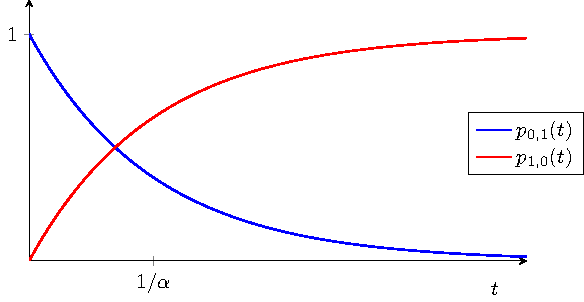
\includegraphics[width=0.62\textwidth]{figures/IMG_ch3/abs1.pdf}
\caption{State probabilities for the single-particle absorption-only model. The particle
begins outside the compartment ($p_{0,1}$, decaying exponentially at rate $\alpha$) and
ends inside it ($p_{1,0}$). There is nowhere else for it to go, so the two curves sum to
one at every time.}
\label{fig:abs1}
\end{figure}

These being the only two non-zero state probabilities of the single-particle system,
\begin{equation*}
G_1(x,y,t) = p_{1,0}(t)\,x + p_{0,1}(t)\,y = \lrb{1-\ee^{-\alpha t}}x + \ee^{-\alpha t}y ,
\end{equation*}
and \cref{eq:indRelPGF} gives the generating function for any initial census,
\begin{equation}
\label{eq:Gabsonly}
G_n(x,y,t) = \Bigl(\lrb{1-\ee^{-\alpha t}}x + \ee^{-\alpha t}y\Bigr)^{n} .
\end{equation}
This satisfies \cref{eq:absPDE1} together with the initial condition $G_n(x,y,0)=y^n$, and
its form is recognisable: $\xt\sim\text{Binomial}\lrb{n,1-\ee^{-\alpha t}}$, as it must be,
since the $n$ particles are absorbed independently and each has been taken up by time $t$
with probability $1-\ee^{-\alpha t}$.

\subsection{Absorption--death}
\label{sec:absdeath}

A particle resident in a compartment may die. Keeping $\xt$ and $\yt$ for the interior and
exterior counts, death enters as a third channel:
\begin{align*}
\pr{\Delta\xx=1,\;\Delta\yy=-1 \;|\; \yt=j} &= j\alpha\delt, &&\text{(absorption)}\\
\pr{\Delta\xx=-1,\;\Delta\yy=0 \;|\; \xt=i} &= i\mu\delt, &&\text{(death)}\\
\pr{\Delta\xx=0,\;\Delta\yy=0 \;|\; \yt=j,\,\xt=i} &= 1-\lrb{j\alpha+i\mu}\delt, &&\text{(no event)}
\end{align*}
with forward equations
\begin{equation}
\label{eq:FK2}
\ddt{\p} = \alpha(j+1)p_{i-1,j+1} + \mu(i+1)p_{i+1,j} - (\alpha j+\mu i)\p .
\end{equation}
The derivation of \cref{sec:absonly} runs unchanged on the extra terms and produces
\begin{equation}
\label{eq:PDE2}
\pddt{G(x,y,t)} = \mu(1-x)\pdd{G(x,y,t)}{x} + \alpha(x-y)\pdd{G(x,y,t)}{y},
\qquad G(x,y,0) = y^N ,
\end{equation}
and the same difficulty. Once again, though, individual particles remain independent in
their movements, so \cref{eq:indRelPGF} still applies.

Without birth events the number of particles cannot exceed its initial value, so for an
isolated particle the generating function has just three terms,
\begin{equation*}
G_1(x,y,t) = p_{0,0}(t) + p_{1,0}(t)\,x + p_{0,1}(t)\,y ,
\end{equation*}
corresponding to a particle that is dead, absorbed, or still outside. The state
probabilities follow from
\begin{equation*}
\ddt{p_{0,1}(t)} = -\alpha p_{0,1}(t),
\qquad
\ddt{p_{1,0}(t)} = \alpha p_{0,1}(t) - \mu p_{1,0}(t),
\end{equation*}
whence
\begin{equation}
\label{eq:absdeathstates}
p_{0,1}(t) = \ee^{-\alpha t},
\qquad
p_{1,0}(t) = \frac{\alpha}{\mu-\alpha}\Bigl(\ee^{-\alpha t}-\ee^{-\mu t}\Bigr),
\qquad
p_{0,0}(t) = 1-p_{0,1}(t)-p_{1,0}(t),
\end{equation}
plotted in \cref{fig:abs2}.

\begin{figure}[H]
\centering
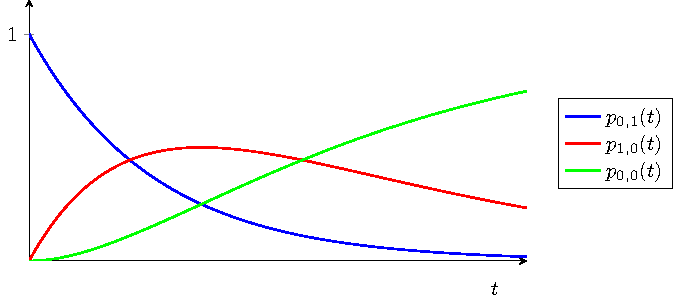
\includegraphics[width=0.62\textwidth]{figures/IMG_ch3/abs2.pdf}
\caption{State probabilities for the single-particle absorption--death model,
\cref{eq:absdeathstates}. The particle starts outside ($p_{0,1}$, blue), is absorbed into
the compartment ($p_{1,0}$, red, which rises and then decays as death takes over), and
finally dies ($p_{0,0}$, green, absorbing).}
\label{fig:abs2}
\end{figure}

Applying \cref{eq:indRelPGF} gives the general generating function
\begin{equation}
\label{eq:Gabsdeath}
G_n(x,y,t) = \Bigl(1-\tfrac{\mu}{\mu-\alpha}\ee^{-\alpha t}
+ \tfrac{\alpha}{\mu-\alpha}\ee^{-\mu t}
+ \tfrac{\alpha}{\mu-\alpha}\bigl(\ee^{-\alpha t}-\ee^{-\mu t}\bigr)x
+ \ee^{-\alpha t}y\Bigr)^{n} .
\end{equation}

\subsection{The method of characteristics, tested on absorption--death}
\label{sec:mocabsdeath}

Before continuing to the case in which replication occurs inside the compartment and the
independence shortcut is unavailable, it is worth revisiting absorption--death from the
point of view of its PDE. Having \cref{eq:Gabsdeath} already in hand makes it an ideal test
case.\footnote{I am grateful to Benjamin Sharp for the advice on applying the method of
characteristics to three-variate problems that unlocked this section.}

Introduce a change of variables $(x,y,t)\to(s,\rho,\tau)$, under which
\begin{equation*}
G(x,y,t) = G\bigl(x(s,\rho,\tau),\,y(s,\rho,\tau),\,t(s,\rho,\tau)\bigr) \equiv G(s,\rho,\tau).
\end{equation*}
The method works by seeking solutions along the characteristic curves of constant $s$ and
$\rho$, on which $G$ is a function of $\tau$ alone. To fix the parametrisation we impose an
initial surface,
\begin{equation}
\label{eq:ICpar}
x(s,\rho,0) = s, \qquad y(s,\rho,0) = \rho, \qquad t(s,\rho,0) = 0 .
\end{equation}
With $G$ a function of $\tau$ only along a characteristic, the chain rule gives
\begin{equation*}
\dda{G}{\tau} = \pddt{G}\dda{t}{\tau} + \pdd{G}{x}\dda{x}{\tau} + \pdd{G}{y}\dda{y}{\tau},
\end{equation*}
which is to be compared with \cref{eq:PDE2} written with everything on one side,
\begin{equation*}
0 = -\pddt{G} + \mu(1-x)\pdd{G}{x} + \alpha(x-y)\pdd{G}{y} .
\end{equation*}
Comparing coefficients yields the characteristic system
\begin{align}
\dda{G}{\tau} &= 0, \label{eq:ch11}\\
\dda{t}{\tau} &= -1, \label{eq:ch12}\\
\dda{x}{\tau} &= \mu(1-x), \label{eq:ch13}\\
\dda{y}{\tau} &= \alpha(x-y). \label{eq:ch14}
\end{align}
Four ordinary \de s have replaced one partial \de{}, and they are solved in the order
written, each supplying what the next needs.

\paragraph{The equation for $G$, \cref{eq:ch11}.}
$G$ is constant along characteristics, $G=\varphi(s,\rho)$. Under \cref{eq:ICpar} the
initial condition $G(x,y,0)=y^N$ becomes $G(s,\rho,0)=\rho^N$, so $\varphi(s,\rho)=\rho^N$
and
\begin{equation}
\label{eq:GrN}
G(s,\rho,\tau) = \rho^N .
\end{equation}
The whole problem thus reduces to expressing $\rho$ in terms of $(x,y,t)$.

\paragraph{The equation for $t$, \cref{eq:ch12}.}
Integrating gives $t = -\tau + c(s,\rho)$, and \cref{eq:ICpar} fixes $c=0$:
\begin{equation}
\label{eq:minustau}
t = -\tau .
\end{equation}
The characteristic parameter runs backwards in time, which is what allows the initial
surface to be reached from any $(x,y,t)$.

\paragraph{The equation for $x$, \cref{eq:ch13}.}
Separating variables gives $1-x = c(s,\rho)\ee^{-\mu\tau}$, and \cref{eq:ICpar} gives
$c = 1-s$:
\begin{equation}
\label{eq:sandxwithtau}
1-x = (1-s)\ee^{-\mu\tau} .
\end{equation}

\paragraph{The equation for $y$, \cref{eq:ch14}.}
Substituting \cref{eq:sandxwithtau} makes the $y$ equation linear,
\begin{equation*}
\dda{y}{\tau} = \alpha\bigl(1-(1-s)\ee^{-\mu\tau} - y\bigr),
\end{equation*}
and solving with integrating factor $\ee^{\alpha\tau}$,
\begin{equation*}
y = 1 - \frac{\alpha}{\alpha-\mu}(1-s)\ee^{-\mu\tau} + c(s,\rho)\ee^{-\alpha\tau} .
\end{equation*}
Applying \cref{eq:ICpar} gives $c(s,\rho) = \rho + \frac{\alpha}{\alpha-\mu}(1-s) - 1$, so
\begin{equation}
\label{eq:ywithr1}
y = 1 - \frac{\alpha}{\alpha-\mu}(1-s)\ee^{-\mu\tau}
+ \lrb{\rho + \frac{\alpha}{\alpha-\mu}(1-s) - 1}\ee^{-\alpha\tau} .
\end{equation}

\paragraph{Recovering the solution.}
Rearranging \cref{eq:ywithr1} for $\rho$, then substituting $s$ from
\cref{eq:sandxwithtau} and $\tau=-t$ from \cref{eq:minustau}, gives
\begin{equation*}
\rho = 1-\frac{\mu}{\mu-\alpha}\ee^{-\alpha t} + \frac{\alpha}{\mu-\alpha}\ee^{-\mu t}
+ \frac{\alpha}{\mu-\alpha}\bigl(\ee^{-\alpha t}-\ee^{-\mu t}\bigr)x + \ee^{-\alpha t}y ,
\end{equation*}
which is exactly the bracket of \cref{eq:Gabsdeath}; substituting into \cref{eq:GrN}
reproduces that solution. The two routes agree, and the machinery is ready for the case
where only one of them is available.

\subsection{Absorption--birth--death}
\label{sec:absbirthdeath}

Introducing replication for particles inside the compartment, we shall see that although
the independence property is still present it no longer serves as a shortcut. Given a
single initial particle, birth events make infinitely many states reachable, so
$G_1(x,y,t)$ is an infinite sum and there is nothing to be gained by factorising. We are
now equipped to solve the PDE directly, and that is the approach taken.

With $\xt$ and $\yt$ as before, birth joins the transition probabilities:
\begin{align*}
\pr{\Delta\xx=1,\;\Delta\yy=-1 \;|\; \yt=j} &= j\alpha\delt, &&\text{(absorption)}\\
\pr{\Delta\xx=1,\;\Delta\yy=0 \;|\; \xt=i} &= i\beta\delt, &&\text{(birth)}\\
\pr{\Delta\xx=-1,\;\Delta\yy=0 \;|\; \xt=i} &= i\mu\delt, &&\text{(death)}\\
\pr{\Delta\xx=0,\;\Delta\yy=0 \;|\; \yt=j,\,\xt=i} &= 1-\lrb{j\alpha+i\mu+i\beta}\delt, &&\text{(no event)}
\end{align*}
with forward equation
\begin{equation}
\label{eq:FK3}
\ddt{\p} = \alpha(j+1)p_{i-1,j+1} + \mu(i+1)p_{i+1,j} + \beta(i-1)p_{i-1,j}
- (\alpha j+\mu i+\beta i)\p .
\end{equation}
The same reasoning as before gives the generating-function PDE
\begin{equation}
\label{eq:PDE3}
\pddt{G} = \lrb{\mu - (\mu+\beta)x + \beta x^2}\pdd{G}{x} + \alpha(x-y)\pdd{G}{y},
\qquad G(x,y,0) = y^N .
\end{equation}
The coefficient of $\partial G/\partial x$ is now quadratic rather than linear, which is
the whole of the additional difficulty. Reparametrising $(x,y,t)\to(s,\rho,\tau)$ as in
\cref{sec:mocabsdeath} gives the characteristic system
\begin{align}
\dda{G}{\tau} &= 0, \label{eq:ch21}\\
\dda{t}{\tau} &= -1, \label{eq:ch22}\\
\dda{x}{\tau} &= \mu-(\mu+\beta)x+\beta x^2, \label{eq:ch23}\\
\dda{y}{\tau} &= \alpha(x-y), \label{eq:ch24}
\end{align}
with the same initial conditions \cref{eq:ICpar}.

\paragraph{The equations for $G$ and $t$, \cref{eq:ch21,eq:ch22}.}
Unchanged from before,
\begin{equation}
\label{eq:GrN3}
G(s,\rho,\tau) = \rho^N,
\qquad t = -\tau .
\end{equation}

\paragraph{The equation for $x$, \cref{eq:ch23}.}
This is a Riccati equation of the same shape as the one governing the survival probability
in \cref{sec:riccati}. Its right-hand side factorises, and it is worth noting that the
roots are elementary rather than the surd expression the quadratic formula appears to
promise:
\begin{equation}
\label{eq:xpm}
\mu-(\mu+\beta)x+\beta x^2 = \beta(x-x_+)(x-x_-),
\qquad
x_+ = 1,\quad x_- = \frac{\mu}{\beta} .
\end{equation}
The discriminant is
$\bigl(\tfrac{\mu+\beta}{2\beta}\bigr)^2 - \tfrac{\mu}{\beta}
= \bigl(\tfrac{\beta-\mu}{2\beta}\bigr)^2$, a perfect square, so the surds cancel. It is
convenient to name the combination that appears throughout,
\begin{equation}
\label{eq:b1}
b_1 = \beta(x_+-x_-) = \beta-\mu ,
\end{equation}
the net interior growth rate. Separating variables in \cref{eq:ch23} and applying
\cref{eq:ICpar} gives the characteristic in the compact form
\begin{equation}
\label{eq:xratio}
\frac{x-x_+}{x-x_-} = \lrb{\frac{s-x_+}{s-x_-}}\ee^{b_1\tau},
\end{equation}
or, solved for $x$,
\begin{equation}
\label{eq:xabd}
x(\tau) = \frac{x_+(s-x_-) - x_-(s-x_+)\ee^{b_1\tau}}
               {(s-x_-) - (s-x_+)\ee^{b_1\tau}} .
\end{equation}

\paragraph{The equation for $y$, \cref{eq:ch24}.}
With an integrating factor the last characteristic equation becomes
\begin{equation}
\label{eq:yint}
\dda{}{\tau}\lrb{\ee^{\alpha\tau}y} = \alpha\,\ee^{\alpha\tau}x(\tau),
\end{equation}
and the integral on the right is where the difficulty lies. Rather than substitute
\cref{eq:xabd} and split the resulting quotient --- which leads to two hypergeometric
integrals and a good deal of bookkeeping --- it is cleaner to expand $x(\tau)$ first.
Writing $x-x_- = (x-x_+)+(x_+-x_-)$ in \cref{eq:xratio} and solving for $x$ gives
\begin{equation}
\label{eq:xgeom}
x(\tau) = x_+ + (x_+-x_-)\frac{\zeta(\tau)}{1-\zeta(\tau)},
\qquad
\zeta(\tau) = \lrb{\frac{s-x_+}{s-x_-}}\ee^{b_1\tau},
\end{equation}
so that, for $|\zeta|<1$,
\begin{equation*}
x(\tau) = x_+ + (x_+-x_-)\sum_{n=1}^{\infty}\zeta(\tau)^n .
\end{equation*}
Every term is now a pure exponential in $\tau$ and integrates immediately. Writing
$Z = (s-x_+)/(s-x_-)$, so that $\zeta(\tau) = Z\ee^{b_1\tau}$ and
$Z^n\ee^{nb_1\tau} = \zeta^n$,
\begin{align*}
\alpha\int\ee^{\alpha\tau}x(\tau)\,\dd\tau
&= \alpha x_+\!\int\!\ee^{\alpha\tau}\dd\tau
 + \alpha(x_+-x_-)\sum_{n=1}^{\infty}Z^n\!\int\!\ee^{(\alpha+nb_1)\tau}\dd\tau\\
&= \ee^{\alpha\tau}\lrbs{x_+ + \alpha(x_+-x_-)\sum_{n=1}^{\infty}\frac{\zeta^n}{\alpha+nb_1}}
 + \text{const}.
\end{align*}
Setting $\delta = \alpha/b_1$ and using $\alpha(x_+-x_-)/b_1 = \alpha/\beta$ from
\cref{eq:b1}, the bracket defines the function that carries the whole solution,
\begin{equation}
\label{eq:Psidef}
\Psi(\zeta) \;=\; x_+ + \frac{\alpha}{\beta}\sum_{n=1}^{\infty}\frac{\zeta^{\,n}}{n+\delta},
\qquad \delta = \frac{\alpha}{b_1} = \frac{\alpha}{\beta-\mu} .
\end{equation}
So $\alpha\int\ee^{\alpha\tau}x(\tau)\dd\tau = \ee^{\alpha\tau}\Psi(\zeta(\tau))+\text{const}$,
and integrating \cref{eq:yint} gives
$\ee^{\alpha\tau}y = \ee^{\alpha\tau}\Psi(\zeta(\tau)) + \text{const}$. The initial
condition $y(s,\rho,0)=\rho$ with $\zeta(0)=Z$ fixes the constant as $\rho-\Psi(Z)$, so
\begin{equation}
\label{eq:rsolved}
\rho = \ee^{\alpha\tau}\Bigl[y-\Psi\bigl(\zeta(\tau)\bigr)\Bigr] + \Psi(Z).
\end{equation}
Finally, put $\tau=-t$ and use \cref{eq:xratio}: writing
\begin{equation*}
W \;=\; \frac{x-x_+}{x-x_-}
\end{equation*}
we have $\zeta(\tau)=W$ and $Z = W\ee^{-b_1\tau} = W\ee^{b_1t}$. Substituting into
\cref{eq:rsolved} and applying \cref{eq:GrN3} gives the solution.

\begin{proposition}[Generating function for absorption--birth--death]
\label{prop:Gabd}
With $x_+=1$, $x_-=\mu/\beta$, $b_1=\beta-\mu$, $\delta=\alpha/b_1$,
$W = (x-x_+)/(x-x_-)$ and $\Psi$ as in \cref{eq:Psidef},
\begin{equation}
\label{eq:Gabd}
\boxed{\;
G(x,y,t) = \Bigl\{\ee^{-\alpha t}\bigl[y-\Psi(W)\bigr] + \Psi\bigl(W\ee^{b_1t}\bigr)\Bigr\}^{N}. \;}
\end{equation}
\end{proposition}

Three checks confirm the result. At $t=0$ the two $\Psi$ terms cancel and $G=y^N$, the
required initial condition. At $x=y=1$ we have $W=0$ and $\Psi(0)=x_+=1$, so $G=1$ and
probability is conserved. And setting $x=1$ alone gives
\begin{equation*}
G(1,y,t) = \bigl(\ee^{-\alpha t}y + 1 - \ee^{-\alpha t}\bigr)^{N},
\end{equation*}
so $\yt\sim\text{Binomial}\lrb{N,\ee^{-\alpha t}}$ --- exactly right, since the exterior
particles are absorbed independently at rate $\alpha$ and what happens inside the
compartment cannot affect them. Beyond these, \cref{eq:Gabd} has been verified numerically
against direct integration of the master equation \cref{eq:FK3}, agreeing to around
$10^{-13}$ across sub- and supercritical interior regimes and for $N=1,2,3$.

\subsubsection*{Hypergeometric form}

The series in \cref{eq:Psidef} is a Gauss hypergeometric function in disguise. With
\begin{equation}
\label{eq:2F1def}
{}_2F_1(a,b;c;z) = \sum^\infty_{n=0}\frac{(a)_n(b)_n}{(c)_n}\frac{z^n}{n!},
\qquad
(q)_n = \begin{cases} 1, & n=0,\\ q(q+1)\cdots(q+n-1), & n\ge1,\end{cases}
\end{equation}
where $(q)_n$ is the rising Pochhammer symbol, the case $a=1$, $b=\delta$, $c=\delta+1$
collapses to a single ratio. Since $(1)_n = n!$ and
\begin{equation}
\label{eq:pochcancel}
\frac{(\delta)_n}{(\delta+1)_n}
= \frac{\delta\cancel{(\delta+1)}\cdots\cancel{(\delta+n-1)}}
       {\cancel{(\delta+1)}\cdots\cancel{(\delta+n-1)}(\delta+n)}
= \frac{\delta}{\delta+n},
\end{equation}
we have
\begin{equation}
\label{eq:2F1simple}
{}_2F_1\lrb{1,\delta;\delta+1;z} = \sum_{n=0}^{\infty}\frac{\delta}{\delta+n}z^n .
\end{equation}
Comparing with \cref{eq:Psidef} and using
$\alpha/(\beta\delta) = b_1/\beta = x_+-x_-$,
\begin{equation}
\label{eq:Psihyp}
\Psi(\zeta) = x_+ + (x_+-x_-)\Bigl[{}_2F_1\lrb{1,\delta;\delta+1;\zeta} - 1\Bigr].
\end{equation}
\Cref{eq:Gabd} together with \cref{eq:Psihyp} is the closed form. It is not pretty, but it
is a genuine closed form in terms of a standard special function, and the elementary series
\cref{eq:Psidef} is what one would actually evaluate. An alternative derivation of the same
object, through the integral $\int\ee^{h\tau}/(P+Q\ee^{k\tau})\,\dd\tau$, is given in
\cref{app:hyp}; that route is longer, but it produces a general identity of independent
use.

\begin{remark}[Domain of validity]
\label{rem:domain}
The series \cref{eq:Psidef} converges for $|\zeta|<1$, and the arguments appearing in
\cref{eq:Gabd} are $W$ and $W\ee^{b_1t}$. In the subcritical interior regime $\mu>\beta$ we
have $b_1<0$ and $x_-=\mu/\beta>1$, so for $x\in[0,1]$ the argument $W$ lies in
$[0,\beta/\mu]\subset[0,1)$ and $W\ee^{b_1t}$ is smaller still: the series representation
is valid on the whole of the unit square, which is the case of most interest here. When
$\beta>\mu$ the series converges only for $x$ above the smaller fixed point $\mu/\beta$,
and elsewhere one must use the analytic continuation of ${}_2F_1$ --- conveniently, the
Euler integral
\begin{equation*}
{}_2F_1\lrb{1,\delta;\delta+1;\zeta} = \delta\int_0^1\frac{u^{\delta-1}}{1-\zeta u}\,\dd u
\qquad (\delta>0,\ \zeta\notin[1,\infty)),
\end{equation*}
which was used for the numerical verification quoted above.
\end{remark}

\begin{remark}[Resonance]
\label{rem:resonance}
The denominators in \cref{eq:Psidef} vanish when $n+\delta=0$ for some integer $n\ge1$,
that is when
\begin{equation*}
\alpha = n(\mu-\beta),\qquad n=1,2,\dots
\end{equation*}
This is the classical resonance condition for linearising the $y$ equation: the homogeneous
decay rate $\alpha$ of the absorption channel coincides with a harmonic of the interior
relaxation rate $\mu-\beta$. The generating function itself is perfectly regular there, being
analytic in all parameters, so the singularity is removable, and at resonance the
corresponding term acquires a factor $\tau$ --- a secular term --- in place of the simple
exponential. The resonant parameter values form a set of measure zero and the limit may be
taken numerically, but the degeneracy is worth keeping in mind when $\alpha$ happens to sit
near an integer multiple of $\mu-\beta$.
\end{remark}

\FloatBarrier
